\section{Current ICME Tools are Well Equipped to Integrate with an ML Framework}
The interdisciplinary nature of AM has naturally led to a compartmentalization of scientific efforts. Since full-scale models of AM are not widespread, many scientists choose to focus on a single problem or process. 

The following section details how machine learning approaches can tie-in to current efforts in AM. Since the study of AM is often focused around specific problems, this section is tailored to many common areas of study within AM. Different methods of analysis and characterization for different aspects of AM all tie-in well with different machine learning algorithms. Even more so, ML can be used to unite knowledge creation across AM's spatiotemporal scales.

%~%~%~%~%~%~%~%~%~%~%~%~%~%~%~%~%~%~%~%~%~%~%~%~%~%~%~%~%~%~%~%~%~%~%~%~%~%~%~%~%~%~%~%~
\subsection{Pre-Build Design}
\subsubsection{Alloy Design}
The additive design process begins with choice of material. The wide swath of additive manufacturing processes \cite{WohlersReport2017} accompanies as many or more choices of material. The choice of metal alloy can dictate the material properties that are obtainable, as well as the final quality of the build. Rapid melting and solidification of powders and feedstock wires is problematic for some alloys. Alloys containing low--vapor pressure constituents---such as aluminum in titanium alloys or magnesium in aluminum alloys---will sometimes vaporize during the manufacturing process, affecting stoichiometry. Some additively manufactured alloys also exhibit microstructures that are conducive to hot tearing upon cooling. Hot tearing is especially prevalent in AM processes because of rapid, non-uniform solidification \cite{Sames2016, Chen2016}. Anisotropic grain growth causes liquid to become trapped in between dendrites, leading to cavities upon solidification \cite{Martin2017}. Alternatively, rapid solidification can also provide unique strengthening mechanisms \cite{Brice2018}. Combining the uniqueness of AM systems with novel alloy choices can uncover new, improved material properties. It also provides an example for applying similarity metrics to optimize the AM process.

In some cases when designing alloys, designers are aware of the requirements necessary for the desired material performance. For example, Martin et al. identified that low energy barrier nucleants need to have minimized lattice strain between nucleating and nucleant crystal structures. In cases like this databases of material information can be algorithmically searched for candidate materials that \textit{at least} match this criteria. Martin completed a search of over 4,500 candidate materials for low energy-barrier nucleants of equiaxed Al-alloy microstructures \cite{Martin2017}. Databases of alloys' crystal structures can be mined for lattice vectors of possible phases. Calculating phase mismatch strain by lattice vectors in a database provides a straightforward, automated measure of how well a possible material might perform. The lattice spacing of a crystal can be described through a vector $\vec{a}$. For any two crystal structures oriented along a given crystallographic direction, with lattice vectors $\vec{a}$ and $\vec{b}$ respectively, will have a strain of
\begin{equation}
	\epsilon = \frac{||\vec{a}|| - ||\vec{b}||}{||\vec{a}||}.
	\label{strain}
\end{equation}
If a researcher investigates $n$ number of candidate materials, then they can calculate $\epsilon_i$ for every possible interface plane between all $i$ phases and the alloy.  If the lattice mismatch is huge between the alloy being manufactured and the nucleant used then the energy barrier to nucleation is large. This similarity metric whittles the candidates down to those with a small lattice strain. Then those materials with the lowest $\epsilon_i$'s are chosen as initial candidates.

%\fig
%\includegraphics[width=1\linewidth]{Images/latdist}
%\caption{Transferring materials information into algebraic structures can open up new searching and classification tools through the use of distance metrics and model fitting. Using these algebraic structures also lends itself to algorithmic computation, with no human intervention.}
%\label{latdist}
%\fiu

The same databases can also contain \textit{other} relevant information about alloy systems, other than just composition and crystal spacing. The electronic properties, chemical properties, and more of different elements have been measured or simulated. In the event that an alloy designer \textit{doesn't} know the necessary conditions for desired performance then the `search' for a new alloy becomes complicated. Typical approaches proceed through trial-and-error evaluation. Adopting machine learning methods to these same databases can improve the trial-and-error process.

%\fig
%\includegraphics[width=1\linewidth]{Images/GA}
%\caption{A good caption goes here.}
%\label{GA}
%\fiu

Even when the exact criteria for design are not known, many materials engineers have analytical or computational models that will estimate alloys' properties from first principles, empirical models, or otherwise. Common examples are density functional theory, molecular dynamics, phase field modeling, and more. An alloy designer can accurately predict the mechanical/chemical/electronic properties of an alloy \textit{if} they have an idea of a starting composition. It follows, then, that one method to find new alloys is run all combinations of compositions through a crucible of models and pick the best one. Of course, running a model through all combinations of elements is not feasible.

In cases like this, machine learning algorithms such as genetic algorithms (GA) can aid in alloy design. The principles of GA are not in measuring similarity of vectors themselves, as done in Eqn. \ref{strain}, but to \textit{transform} those vectors and assess their similarity to an optimization condition. The manner of transformation is typically restricted to a set of given mathematical operations.

We have a database of compositions $\chi_i$ , and their associated atomic or material properties $\vec{x}_i$. We also have a currently-existing model that can predict, within a given accuracy, the properties of an alloy $\vec{y} = f(\chi_i, \vec{x}_i) = f(\chi_i,x_1,x_2,...,x_n)$. An alloy designer would like to use this model to inform design decisions, but does not have the time to assess $f(\cdot)$ at all points in the design space. 

Genetic algorithms can operate on the \textbf{inputs} of models in order to search design spaces for the optimal inputs to achieve a desired output. For example, we may want to maximize a certain material value $y$. We can start with two samples from the input space $(\chi_1,\vec{x}_1)$ and $(\chi_2, \vec{x}_2)$. Then, the model would be run and assessed to estimate the parameter $y$. Whichever input produced a higher value for $y$ would be kept, while the other input can be discarded from the set of possible candidates.

Now, a new set of inputs is chosen to be explored, $(\chi_3,\vec{x}_3)$ and $(\chi_4,\vec{x}_4)$. The same process is repeated -- whichever input produced a better result is kept, while the other is discarded. The designer is now left with two possible inputs -- let's say $(\chi_1,\vec{x}_1)$ and $(\chi_4,\vec{x}_4)$ -- that produced better results than their competitors. By relying on the locality hypothesis the designer can say that these inputs are closer to optimal points in the design space than other input choices. Other optimal choices might be near these. The task still remains to find the \textit{best} input in the design space.

Genetic algorithms find these local regions of optimality by operating on those inputs which are `best' by the model's choice - in this case $(\chi_1,\vec{x}_1)$ and $(\chi_4,\vec{x}_4)$. To find \textit{better} inputs the designer can look near these initial guesses. A series of operations on $(\chi_1,\vec{x}_1)$ and $(\chi_4,\vec{x}_4)$ can produce inputs in the neighborhood of the original chosen inputs, but might be better. Operations in a genetic algorithm are often described analogously to mutation and crossover in genetics. Various elements comprising $\chi_1$ and $\chi_4$ could be interchanged, or they could be alloyed together into a new composition $\chi_1 + \chi_2$. A single element in the composition could be added or deleted. The quantified material properties could be altered $\vec{x}_1 + \epsilon$ to see if they improve stability. Once mutations are made to the alloy `gene,' the new composition or properties are assessed by a model $f(\cdot)$ to determine if they move closer to design optimality or further away. If they move closer, further mutations may be performed to attempt to move even closer. If the result is less optimal, new compositions and associated properties may be chosen, compared, and the better result may be genetically modified.

Having a tool such as a predictive model $f(\cdot)$ is useful in cases where the model inputs are known. It would be just as useful to have a tool that points us toward the right inputs to achieve our desired output. Genetic algorithms use models to provide such a tool by cleverly iterating through design space possibilities. Furthermore, genetic algorithms provide an interpretable method of searching through our design spaces while also screening out highly unlikely candidate materials. So long as a designer has a measurable optimization criteria -- say the Hall-Petch equation, for example -- they can employ GA's to search for the right material. In the case of Hall-Petch, the designer may be looking for an alloy with minimized grain size. A genetic algorithm could be trained to optimize the inputs of the model, specifically the composition of the alloy solidifying. 

Genetic algorithms have been applied to alloy design for low and high temperature structural materials \cite{Ikeda1997, Kulkarni2004}, ultra high strength steels \cite{Xu2008}, specific electronic band gaps \cite{Dudiy2006}, minimum defect structures \cite{Mousavi2006}, exploring stable ternary or higher alloys alloys \cite{Hautier2010, Johannesson2002}, and more. For a review on the application of GA's to alloy design through the early 2000s see Ref. \cite{Chakraborti2004}.
 

%\fig
%\includegraphics[width=1\linewidth]{Images/enthalpy}
%\caption{The enthalpy of formation is lowest in certain regions of the crystal lattice space, indicating that this trend follows trends in composition. Image taken from Ref. \cite{Johannesson2002}}
%\label{enthalpy}
%\fiu

%~%~%~
\subsubsection{Design of Experiments}

In alloy design, as with many different engineering methods, repeated trial of new samples is required to validate the predictions of any model. Ideally, experimentalists will obtain the necessary level of confidence in their prediction with \textit{as few tests as possible}. Many different approaches exist for finding this path including traditional design of experiments, latin hypercube, and more. These approaches maximize the information gained from each test. A litany of machine learning approaches exist for the same purpose, with added functionalities \cite{Shan2010}. Many of these machine learning approaches are based on assessing the impact of a single input $x$ on the prediction power of a given model $f(\cdot)$. 

Say, for example, that a researcher has a property $y$ of interest that \textit{may be} dependent upon one or more parameters from a set $\{x_i\}$. In the case that the range of each $x_i$ is large or the parameter set size $n$ is large, or both, the combinatorial problem of characterizing $y$'s dependence upon $\{x_i\}$ becomes tedious, time-consuming, and expensive. Running a full-factorial design of experiments may be out of the question.

Instead, a researcher can rely on statistical analysis to provide robust information with as few tests as possible. The experimentalist may have a subset of data, either personally obtained or published, $\{\mathbf{y_{\text{sub}}}\}$ that were measured for a small set of manufacturing conditions $\{x_\text{sub}\}$. This means a simple model can be assessed such as 
\begin{equation}
	\mathbf{y}_\text{sub} = f_1 (x_\text{sub})
	\label{model1}.
\end{equation}
An important feature of any model is its error in prediction. One way to assess this error is through a distance measurement, such as
\begin{equation}
	\epsilon = ||\mathbf{y}_\text{sub} -f_1 (x_\text{sub})||
	\label{model1eps}
\end{equation}
where $\epsilon$ is referred to as the residual of the model. If we wanted to study the predicted value of a specific input $x^*$ then we may evaluate Eqn. \ref{model1eps} at $f(x^*)$ and observe the residual. 

In the event that $\epsilon$ is small then the predictive power of $f_1$ in that regime is high. However, if $\epsilon$ is large then it may indicate that we do not have enough input data for $\mathbf{y}$ and $x^*$ in that region of the design space. Thus, we should run more tests at a range of values similar to $x^*$. This type of sample selection criteria is known as maximum uncertainty. 

When performing searches for maxima/minima of quality in manufactured parts this analysis enables faster searching of the design space than random sampling, or even informed experimental design in some cases. If an engineer is given a material property to optimize, like tensile strength, elongation, hardness, fatigue life, etc., then they can choose to manufacture parts at a range of conditions. The exact relationship between the property and the manufacturing conditions is unknown - in fact, the engineer may be characterizing this property for the first time. However, they would still like to reach an optimized condition in as few experiments as possible. 

The above experimental setup is the premise of a study completed by Ling et al., that assessed maximum uncertainty criteria, among others, for four different materials datasets. When comparing four different statistical methods of sample selection sampling, they were able to reach an optimized condition with up to 221 \textit{fewer} samples than random sampling \cite{Ling2017}. When taking into consideration the costs of performing experimental analysis, whether it is sample manufacturing, sample preparation, machine operation, person hours, a reduction of 221 samples can make a major difference.

\subsubsection{Topology Optimization}
Alloy and experimental design and optimization focuses around combinatorial screening of inputs to either search for \textit{new} properties or optimize on current properties. These optimizations focus around reducing manufacturing cost, monetary or otherwise, and maximizing performance capability. The same optimization can be applied to mechanical properties of parts. In the mechanical case, the goal would be to optimize load bearing capacity or lifetime while minimizing the amount of material used. A solid block of AMed steel could likely act as a structural part; a truss would probably get the same job done with considerably less material.

Topology optimization (TO) focuses around exactly this task -- finding optimized topological structures for a given mechanical application. TO takes advantage of many breakthroughs promised by additive manufacturing. The unique manufacturing ability of AM means that otherwise un-machinable metal parts can be produced ergo unique structural geometries with optimized mechanical responses can be engineered. 

The basic premise of TO is applying filters to pixelized/voxelixed mesh representations of continuum parts. Convolutional filters pass over regions of voxels and minimize the number of voxels needed to meet an optimization criterion by selectively removing material and calculating the mechanical response in return. 


Topology optimization algorithms have been developed specifically for additive maufacturing. Additive-specific design concerns can invalidate the results of optimization algorithms or produce unrealistic manufacture conditions. Some examples include limitations on the angle at which a part can be printed. An unsupported slope at acute angles can lead to part deformation and warpage \cite{Gaynor2016}. Sacrificial support structures also need to be considered during topological optimization, along with the number of free-hanging features and the orientation of the part during manufacture \cite{Langelaar2016}. 

These additive-specific TO algorithms are actually indicative of a larger problem. Many different models exist for many different aspects of additive manufacturing. Knowledge transfer between models is not always possible, or even obvious in its implementation. A key need for the field is a comprehensive model which incorporates all relevant physics that might impact a part's final performance. The success of such a model is limited by our ability to understand how physics at different spatiotemporal scales interact.
%~%~%~

%~%~%~%~%~%~%~%~%~%~%~%~%~%~%~%~%~%~%~%~%~%~%~%~%~%~%~%~%~%~%~%~%~%~%~%~%~%~%~%~%~%~%~%~%
\subsection{Process Design}
An ideal model of the additive manufacturing process would take as input an alloy, a CAD model, and a list of manufacturing parameters and return the likely material properties of the final part. A better model of the additive process would also take as input an alloy, a CAD model, and a list of material properties to optimize and return the necessary manufacturing parameters. Achieving either one of these models is dependent upon knowledge transfer between currently existing, sub-physics models. 

The additive process is currently studied through a variety of computational lenses. Some models focus on single phenomena, such as powder flowability, laser-powder interactions, melting and re-solidificaiton, fluid flow in the melt pool, phase formation during solidification, heat transfer, and more. Some models incorporate several physical phenomena and study their interaction or impact on the part, such as full-physics simulations of laser keyholing \cite{King2014}. Still, a model that incorporates all necessary physics is desired. 

The road to a comprehensive model requires several key advancements, including
\begin{itemize}
	\item Computationally accessible sub-physics models
	\item Knowledge transfer methods between sub-physics models
	\item Many-parameter empirical models
\end{itemize}
as well as other need areas of additive manufacturing modeling \cite{King2015b}. These areas can be tackled, in kind, with machine learning applications.
	
	
\subsubsection{Reducing Computational Complexity}
Models of physical phenomena often begin with first principles, such as Newton's second law, Fourier's heat transfer equation, the Maxwell Equations, Schr\"odinger's equation, and the list continues. Terms in each equation are then expounded upon, incorporating other physical models of forces, energies, potentials, and more. The computational expense of a model is determined by how much physics is incorporated and the resolution at which the problem is modeled, among many other considerations. One workaround is better computers that can handle a larger I/O stream. Another approach is reduce the number of operations performed while still achieving a good enough description of the underlying physics.

Scientific endeavors are focused around descriptions of physical phenomena that are as accurate as possible. From an engineering and process modeling perspective, having a model that is `good enough' at modeling the phenomenon suffices. In this case, `good enough' means the model makes accurate predictions for the engineering application. Currently existing computational models can be downsized to be just `good enough' by analysis of which physics actually need to be incorporated to accurately predict the final result. 

A combinatorial approach can be employed to determine the most important inputs of a simulation by iterating through many possible manufacturing conditions and evaluating the difference in results. Many simulations can be run and then analyzed for conditions such as computation time or accuracy with experimental results. Similarly, running a test matrix of manufacturing conditions can also give insight to the \textit{best} conditions for a desired part property, like density. Kamath et al. applied a random forest algorithm to both of these ends. Their goal was to find the most important manufacturing conditions impacting melt pool depth and predict the best melt pool conditions to produce fully dense 316L stainless steel parts. To understand why Kamath's study was successful, it is necessary to understand the basics of random forest algorithms. 

Two key strengths of the random forest algorithm are its ease of use and its quick training time. Random forests are easy to use because they do not require tuning many hyper-parameters. Furthermore, random forests are very good at sifting through many irrelevant features to find the features that actually matter. They do not require data scaling or feature selection. Random forest training is also computationally inexpensive and easily parallelized. Random forests provide two advantages that are particularly important in the context of materials science: the ability to efficiently calculate uncertainty estimates and the added interpretability of feature importance metrics. Based on their ensemble nature, it is possible to generate uncertainty estimates for random forest predictions using jackknife-based procedures~\cite{Efron1992, Efron2014, Wager2014}. While uncertainty estimates are not needed in many mainstream machine learning use cases, they are critical in many materials science applications. Random forests also provide more interpretability than other machine learning methods. They automatically identify the most important features in a given model based on how often a feature is used in splitting criteria and what the aggregated information gain is over those splits. These feature importance metrics can provide insights into how the model is making its predictions. 

%\begin{figure}[t]
%\begin{center}
%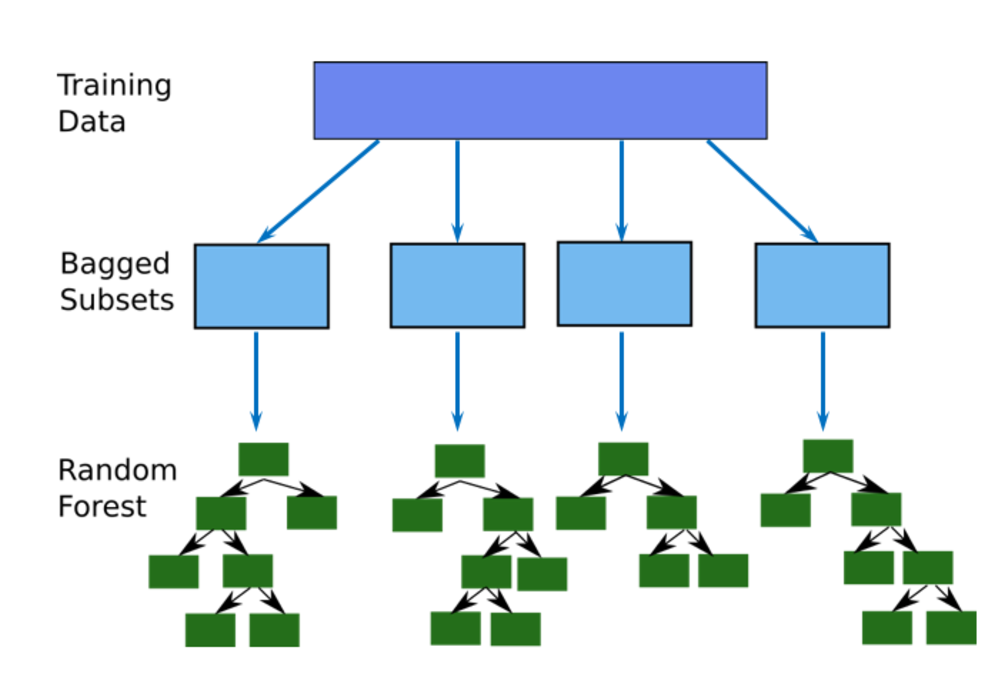
\includegraphics [width=65mm]{Images/randomforest2.eps}
%\end{center}
%\caption{Schematic of the random forest algorithm. The training data are randomly subsampled via bagging, and each bag is used to train a decision tree. All trees have an equal vote toward the final prediction.} 
%\label{fig:randomforest} 
%\end{figure}

Random forests have been applied successfully to a range of applications in materials science. They have been used to discover new Heusler compounds~\cite{Anton} and new thermoelectric materials~\cite{Gaultois}. They have also been used to model material properties such as thermal conductivity in half-Heusler semiconductors ~\cite{Carrete} and to break down fields for dielectrics~\cite{Kim2016}. Ling et al.~\cite{Ling2017IMMI} demonstrated how random forest models with jackknife-based uncertainty estimates could be used for experimental design in materials science. The application of machine learning for experimental design is particularly compelling for AM, where there are many processing steps that affect build quality. 

Kamath utilized random forests among other machine learning techniques to predict melt pool depths based on the results of an Eagar--Tsai model for powder melting \cite{Kamath2016}. The Eagar--Tsai model uses a Gaussian laser beam incident on a metal substrate and models the temperature distribution throughout a bed of powder. Kamath was seeking to understand the most important laser parameters to use for predicting a melt pool's size and shape. Kamath started with the inputs of the Eagar--Tsai model and ordered them based on their numerical value. Then, a random forest algorithm was built that split variables based on the standard deviation of their associated output. The main idea was that variables that had a high impact would have a low standard deviation in their associated outputs. Using this method, they found that laser speed and power were the most important inputs for determining the melt pool depth and shape. After determining the most important inputs, the same regression tree was applied in order to find optimized manufacturing conditions for fully dense parts, using the same method.

Kamath's study also highlights a theme across studies of AM: the process combines separately known physics across separate domains. For example, a laser physics model will have a set of descriptors for describing the laser's behavior, while a solidification model will have a separate set of descriptors for itself. Descriptions across separately contained models do not obviously demonstrate how the descriptors interact, or which descriptors from one model are important to include in the other model. Science has long benefited from simple models, possibly empirical, which provide a small amount of physical descriptors to model specific properties. Machine learning algorithms can search through physical parameters used to model AM to find the lowest dimensional description which explains the widest swath of phenomenon. This is desirable for building computationally accessible models.

The many different computational models of AM, whether they are finite/direct element, central difference, phase field, or otherwise can all be upscaled to describe more and more physics.  Interaction potentials between forces during manufacturing can be added to models, requiring more input descriptors. Take, for example, a finite element model that describes thermal flux through a system from the interaction of a laser on a powder bed \cite{Khairallah2016}. There are many physics to consider here -- the energy transfer of the laser on the powder bed, movement of powder, phase change from powder to melt pool, thermal fluid mass transfer in the melt pool, convective, cooling, and radiative heat loss, and more. The full-physics model may have \textit{many} inputs $\mathbf{x} = (x_1,x_2,...,x_n)$ where $n$ is large.

The original, full-physics model produces a relationships $y = f(\mathbf{x})$ and may be computationally expensive, creating a bottleneck for process design and knowledge generation. A more computationally accessible model $y^*(\mathbf{x^*})$ would be desirable. In this case, the set of descriptors $\mathbf{x^*}$ consists of a subset of descriptors from $\mathbf{x}$, but is a much smaller set and requires less computational resources. 

Stated otherwise, the goal is to solve the objective function
\begin{equation}
	\text{min} ||y^*{(\mathbf{x^*})} - y(\mathbf{x})||
	\label{obj}
\end{equation}
such that $\{\mathbf{x^*} = \left(x_i...x_m\right) \in \mathbf{x} | m << n\}$

Finding the solution to Eqn, \ref{obj} can be achieved by fitting random sampling of descriptors from $\mathbf{x}$ and creating regression models on the outputs of the original model $y(\cdot)$. Presumably, the original full-physics model has been run and evaluated for accuracy. This means the researcher has a set of computationally-generated data $y$ as well as the inputs used to assess the model $\mathbf{x}$. 

Various subsets of the model inputs $\mathbf{x^*}_i$ can be chosen by randomly sampling the full list of inputs $\mathbf{x}$ repeatedly. Each subset of inputs can then be regressed upon, perhaps by using least squares regression
\begin{equation}
	\text{min} ||\mathbf{Y} - \mathbf{X^*_i} \mathbf{c_i}||
	\label{obj2}
\end{equation}
where $\mathbf{Y} = (y_1,y_2,...,y_n)$ are the outputs of the full-physics model, $\mathbf{X} = \left[ \mathbf{x^*} ,\mathbf{x^*},...,\mathbf{x^*}\right]^T$ is an $n \times m$ matrix of the subset of inputs, and $\mathbf{c}$ is a vector of weighting coefficients. This produces a randomly-generated model $y^*(\mathbf{x^*_i}) = \mathbf{X^*_i}\mathbf{c_i}$ which may or may not be able to accurately reproduce $y(\cdot)$. To find the \textbf{best} subset of inputs, one can solve 
\begin{equation}
	\underset{\mathbf{c}}{\text{min}}|| \mathbf{Y} - \mathbf{X^*_i} \mathbf{c_i}|| + \lambda||\mathbf{c_i}||
	\label{KRR}
\end{equation}
which is the objective equation for a machine learning method known as Kernel Ridge Regression (KRR). The idea behind Eqn. \label{KRR} is that it is a feasible minimization problem from a complexity perspective, i.e. it is convex. KRR is the basis of a descriptor set investigation performed by Ghiringhelli et al. to find the lowest dimensional descriptor for predicting crystal structure.They were able to identify one-dimensional, two-dimensional, and three-dimensional descriptors that were all shown to be the ``best'' combinations of descriptors out of any $n$-tuple \cite{Ghiringhelli2015}. Better physical descriptors are often found by combinatorial analysis of as many independent variables and dependent variables as possible. The `best' descriptors found experimentally are usually judged based on the amount of physics they are able to reproduce. Using descriptor analysis, as Ghiringhelli did, experimentalists can find the best descriptors as quickly as possible. Then, when trying to predict material properties in the future, researchers know which descriptors to use or combine.

\subsubsection{Knowledge Transfer Between Single-Physics Models Through Fingerprint Descriptors}
Consider briefly the amalgamation of all empirical models, computational modeling techniques, and first-principles physics representations used to study the AM process. Empirical models can include classical materials science design principles, like the Hall-Petch relationship for grain size and strength \cite{Martin2017}, or even additive-specific empirical models \cite{Gockel2013, Beuth2013}. Computational modeling techniques span a wide range of approaches, including finite element models \textbf{cite}, discrete element models \textbf{cite}, phase field modeling \textbf{cite}, and more. A review on finite element methods specifically for additive can be found at \cite{Gouge2018}.

Current integrated computational models link phenomena across spatiotemporal scales by running many single-physics models and passing the results from model to model, then comparing with experimental results. An example is the model of Martukanitz et al. that considered the thermal, mechanical, and material response of Ti-6Al-4V alloys manufactured with powder bed processes \cite{Martukanitz2014}. Martukanitz's model uses the finite element method to model the thermal and mechanical response based on classical continuum heat transfer equations. At the same time, the Calculation of Phase Diagrams (CALPHAD) method to model the thermodynamics and mass transfer for each chemical species, while Diffusion-Controlled phase Transformations (DICTRA) is used to model phase formation. As noted by Martukanitz, this approach becomes computationally infeasible as the number of deposition layers increases.

Even a \textit{single} modeling method -- just FEA, phase field, CALPHAD, etc -- becomes computationally expensive for thousands of layers of material deposition. Based on this scaling, accurately predicting the final properties of a full build seems impossible, at least without a major leap in computing power. A machine learning method known as \textit{committee voting} or \textit{ensemble modeling} may provide a workaround. These methods rely on sampling many individual, sub-physics models to predict the behavior of a larger class of physics.

In traditional ensemble modeling approaches, many different regression models are trained to model a relationship $y = f(\mathbf{x})$, all trained on different subsets of the data. For a given input $\mathbf{x_1}$ all regression models are assessed and various outputs predicted, $f_1(\mathbf{x}), f_2(\mathbf{x}), ..., f_n(\mathbf{x})$ out of $n$ many models trained. These data sets for additive may be the inputs and solutions of a solidification or heat transfer model, or experimentally obtained relationships.

The ensemble method relies upon taking a vote from the results of all models, either by picking the solution that was guessed the most or taking the average of solutions, or something else. In the AM case, where models may overlap or have experimental data associated with them this type of approach can screen out noise from simulations or experiments to gauge a more fundamental relationship. The uncertainties associated with a model -- models are, after all, only partially representative of reality -- can be weighted by the experimentally observed data points. Furthermore, predictions can be made across many different physical models, resulting in a predictive method for holistic analysis of the final properties.

Meredig et al. applied this method to the prediction of ABC (ternary) compounds \cite{Meredig2014}. Instead of running high-throughput DFT simulations on the combinatorial space of all possible ABC compounds, they used lower order simulations. Tests were run for AB, AC, and BC compounds to predict the formation energies of ternary compounds.

The results of these simulations can then be used as fingerprint descriptors for predicting the results of more complicated interactions, as shown by Meredig et al. For example, classification and regression algorithms can be trained on previously run simulations in order to learn which physical phenomena impact the formation of certain defects. Predictive algorithms can then be used to interpret how the combination of these individual results might impact the overall physics of defect formation, such as keyhole porosity. This is done using metrics of distance, as discussed earlier. 

Of course, we are not limited to statistical sampling of computational models alone. Statistical sampling of a wide enough swath of empirical results can also produce robust results. 

\subsubsection{Surrogate Modeling}

If the criterion for model success is prediction accuracy, then we are not limited to physics-based computational models for data mining. Applying machine learning to a multitude of data -- empirical and computational -- can sample and predict results just as well. A \textit{surrogate model} is a mathematical approximation that can take inputs to numerical simulations and predict the results of a simulation, without actually performing the computation \textbf{\textit{or}} take the independent variables of an experiment and predict measurement values. This is done through statistical sampling of previously run models/experiments, analogous to the manner in which Kamath et al. utilized random forests, or how lower order models can be used to predict the results of higher order models. They have the added benefit of use for inverse design of materials or manufacturing conditions. 

Tapia et al. built a surrogate model for laser powder fusion of 316L stainless steel. They were concerned with predicting the melt pool depth of single-track prints solely from the laser power, velocity, and spot size \cite{Tapia2017}. Data were taken from several different sources. A few datasets were computationally derived, based on previous simulation methods used by the same research team \cite{King2014, Khairallah2016}. They ran powder bed simulations at various laser powers, velocities, and spot sizes, and the model told them the depth of the melt pool, among other information. Their dataset also included some experimentally obtained values of the same information. The combination of these datasets provided enough information for the surrogate model to search a combinatorial design space of manufacturing conditions in a wide enough scope to find local maxima of quality.

To build this model, Tapia et al. used a regression model known as a Gaussian process model (GPM). All data in a GPM is assumed to be evenly distributed in a multivariate normal manner. As with many machine learning models, trends in inputs and outputs in a GPM are elucidated through the covariance of the dataset. Starting with the covariance of their inputs, Tapia et al. used Bayesian statistics to develop a probabilistic model that predicted melt pool depth for the given input parameters. They were able to successfully predict the outcomes of both high-fidelity simulations and experimental measurements solely by analyzing trends in previously obtained results. In particular, they were able to accurately predict the melt pool depth at a value that had never been observed before, either computationally or experimentally. 

%~%~%~%~%~%~%~%~%~%~%~%~%~%~%~%~%~%~%~%~%~%~%~%~%~%~%~%~%~%~%~%~%~%~%~%~%~%~%~%~%~%~%~%~%
\subsection{Process Monitoring and Characterization}
There is an outstanding need to incorporate information gained about AM from the machine learning approaches discussed above into the manufacturing process. There are already many critical design criteria that AM users are aware of, such as constraints on free standing structures \cite{Gaynor2016}, the impact of particle characteristics on quality \cite{Deng2018, Ziolkowski2014}, the interaction of energy density with pore formation \cite{King2014, Cherry2015}, and more. These considerations and constraints need to be incorporated and monitored in situ to ensure final part quality. 

Machine learning can also be adopted for in situ process monitoring and characterization, with multiple possible applications. Some of the most promising applications include automated computer vision monitoring of powder beds for the identification of defect formation, feedback and control mechanisms, and ex-situ image classification of microstructure images.

\subsubsection{In Situ Automated Feature Detection}
Thus far, in situ control in AM has been consistently ranked as one of the most-needed technologies for advancing the technology \cite{Mani2017, Tapia2014}. If the ideal conditions under which to perform manufacturing can be understood, monitoring the process will ensure the desired conditions are achieved. Or, the conditions under which certain defects form could be ascertained. In this case scientists would want to be able to detect the onset of those conditions to adjust the heat source parameters and fix the problem. All of this will require in situ sensing and a level of robotic control. 

A study by Gobert et al. investigated using X-ray CT data to correlate with images obtained by a DSLR camera during the printing process. Gobert et al. printed a single part, containing several different features, and recorded the print results before and after every layer using a DSLR and eight different lighting conditions. The part was then characterized using X-ray CT to find the location and size of pores and inclusions. A matrix list of pixel intensities $I(x,y,z)$ was convolved using a Gaussian blur, whereby each CT image slice was iteratively blurred in order to increase the contrast of differently sized features. This same type of blurring is common in many image recognition algorithms for images with multiple features of varying size \cite{Lowe2004, Bay2008}. The result of the Gaussian blur identifies pixel intensities as high-intensity pixels (inclusions) or low-intensity pixels (voids), with the remaining identified as part of the bulk. Clustering with $k$-means was then applied to group pixels into single pores.

The information from the convolution operation was then used to train an algorithm that detects defect formation from the DSLR results. One of the underlying assumptions of the study was that, even though the DSLR images did not record during the melting and solidification process, features would appear in each image that could be correlated back to the higher-resolution data in the CT images. The DSLR images were projected into the feature space of the convolved CT data using an affine transformation through linear least squares. This transformation provides a mapping by which \textit{new} image data can be mapped to the feature space, giving an estimate of whether or not the new image contains a defect or not. The study by Gobert et al. was able to accurately predict whether or not an image contained a defect with 85\% accuracy after all the DSLR lighting conditions were combined into an ensemble classifier. Similar studies have also achieved good prediction accuracy for AM using convolutional neural networks \cite{Scime2018} and dictionary methods \cite{Abdelrahman2017}. Kernel ridge regression was implemented successfully for fault detection in general manufacturing systems \cite{Wang2018}.

With this type of in situ image recognition, defect formation can be detected during the printing process, precluding the need for certain post-characterization techniques. If defects form and are detected, then the printing process can be stopped, saving powder/feedstock, operating costs, and operating time. However, an even more desirable result is to first detect defect formation, then correct for it in situ. To do so, information will have to be assembled that relates the detection of defects, the manner in which the defects formed, and the prescribed fix to undo or stop the defects from growing. It is likely that combining all these information sources will require a significant leap in scientists' ability to apply machine learning algorithms to widely varying data sets and types. \newline 

\subsubsection{Featurization of Qualitative Image Data}
Images of material microstructures are widespread, (relatively) easily produced, and one of the most important ways that material scientists synthesize material information across domains. There is much important information which can be contained in an image: grain sizes and morphology; texture; retained phases and orientations; presence of defects; surface roughness; and more. All of these parameters are important to a material scientists' intuition. These images are also a common method of studying the final state of additively manufactured parts.

The intuition gained from human interpretation of images is not always encodable in a way that is compatible with models. A human might make a complicated interpretation of an image, such as ``the microstructure is mostly acicular, with some prior grains present, and a string of pores near the boundary." Surely, such a description conjures an image in the reader's head of what such a microstructure might look like. Encoding the same information into a finite element mesh of a microstructure isn't necessarily straightforward. It can be accomplished, for sure, but transforming an observed microstructure into quantitative information requires time-consuming methods.

Image recognition algorithms are making strides at automating quantification of information from images, while also being able to produce qualitative descriptions of the images. Information such as the size of grains, orientation of grains, presence of cracks or pores, different phases, and more can be automatically identified through computer vision. DeCost et al. have made strides in turning metallographs into sets of quantitative information \cite{DeCost2015, DeCost2017, DeCost2017a}. 

In one particular example, DeCost et al. utilize scale invariance feature transform (SIFT) in order to identify possible features in images. The SIFT algorithm is a widely used algorithm for feature identification and is implemented in many open-source packages, such as OpenCV for C++ or Python \textbf{cite OpenCV}. SIFT relies on identifying regions of maximal and minimal intensity in successively blurred versions of an image. The gradient of pixels are regions of extremal intensity are then computed, resulting in a keypoint descriptor which encodes the size and orientation of a feature, as well as generates a descriptor for identifying that object. The idea behind SIFT is that similar features across images will have similar descriptors. This way, common features can be identified across images.

DeCost et al. performed SIFT on a database of microstructure images across several alloys \cite{DeCost2015}. The ``features'' that were identified across \textit{all} images were then clustered by $k$-means clustering to identify a dictionary of features. Human investigation can assign qualitative labels to clusters, such as ``$\alpha$ grain" or ``pore" or ``grain boundary." Now, new images can be analyzed with SIFT and their features can be compared to the dictionary of human-interpretable feature descriptors. 

Not only does this process partially automate analysis of images it also automates translation of image-level information into quantitative information. Grain size can be measured by the number of pixels in an identified grain. Orientation of grains can be determined from the values of the keypoint descriptor. The number of pores in an image can be counted as the number of features which match ``pore" in the dictionary. Of course, a human could perform all of this with a ruler and their eyes. However, a computer can perform the same process much faster and on many more images.

Chowdhury et al. took a more expansive approach to performing feature identification in microstructures. In particular, they were looking to classify microstructures as either dendritic or non dendritic. Chowdhury employed 8 different feature identification methods for a dataset of images. Classification was performed using support vector machines (SVM), Na\"ive Bayes, nearest neighbor, and a committee of the three previous classification methods \cite{Chowdhury2016}. Chowdhury's wide approach to image classification compared the predictive ability of all combinations of feature identification and classification methods, achieving classification accuracies above 90\%.

Chowdhury's study illustrates the depth of machine learning as a discipline and the many, many, many possible implementations which \textit{could} be adopted for different tasks in additive manufacturing. This review is only a brief introduction to the power of statistical analysis methods in materials science. 


%
%\begin{itemize}
%	\item Long and Kusne Example (possibly delete?)
%\end{itemize}
%Common characterization techniques used for AM metals, like X-ray diffractometry (XRD), mechanical testing, composition mapping, and electron microscopy are time-consuming and costly, leading to protracted experimental and analysis cycles \cite{Ziolkowski2014}. 
%
%This type of process is ideal for studying newly observed systems, especially in cases where there is uncertainty about all the phases or structures that might be present. In such cases, a latent variable analysis tool can give approximations of the determining factors that underlie a process, property, or structure. It also enables the search for specific properties in a more informed manner. Kusne et al. applied a clustering method similar to Long's method for the same Fe-Ga-Pd ternary system \cite{Kusne2015a}. They were searching for a candidate material that exhibited magnetic anisotropy and was free of rare-earth elements. By applying mean shift theory---a preprocessing technique like NMF that clusters data into lower dimensional descriptor sets---they were able to quickly identify composition boundaries for phases in this ternary system. From there, a GA approach was used to find the best candidate material. They ended up finding a novel phase that exhibited the property of interest. This approach had proven to be somewhat successful in previous investigations of phase identification for multistructure systems \cite{Serra2007}. Deconvolving material information into basis vectors that can produce structural information is ideal because it also implicitly unlocks information about aspects of property space. 


